\documentclass{article}

\usepackage{lipsum}
\usepackage{geometry}
\usepackage{hyperref}
\usepackage{xcolor}
\usepackage{graphicx}
\usepackage{cleveref}
\usepackage{listings}
\usepackage[framemethod=tikz]{mdframed}
\usepackage{bold-extra}

% links
\hypersetup{
  colorlinks=true,
  linkcolor=red,
  urlcolor=blue
}



% abbreviations
\newcommand{\eg}{\emph{e.g.}}
\newcommand{\ie}{\emph{i.e.}}
\newcommand{\cfr}{\emph{cfr.}}
\newcommand{\etc}{\emph{etc.}}



% custom colors
\definecolor{mygreen}{rgb}{0, 0.6, 0}
\definecolor{myllgray}{rgb}{0.95, 0.95, 0.95}
\definecolor{myddgray}{rgb}{0.25, 0.25, 0.25}
\definecolor{myblue}{rgb}{0, 0.3, 0.8}


% environment for C++ code
\lstdefinestyle{mycpp}{
  basicstyle=\small\ttfamily,
  %frame=single,
  language=C++,
  %backgroundcolor=\color{myllgray},
  commentstyle=\color{mygreen},
  keywordstyle=\color{myblue},
  numbers=left,
  numbersep=5pt,
  numberstyle=\footnotesize\color{black},
  %stringstyle=\color{orange},
  showstringspaces=false,
  xleftmargin=.05\textwidth,
}



% environment for bash/terminal code
\lstdefinestyle{myterm}{
basicstyle=\small\ttfamily,
%language=bash,
commentstyle=\color{mygreen},
keywordstyle=\bfseries,
numbers=none,
showstringspaces=false,
xleftmargin=.5\parindent,
}



% environment for CMake code
\lstdefinestyle{mycmake}{
  basicstyle=\small\ttfamily,
  %frame=single,
  %backgroundcolor=\color{myllgray},
  commentstyle=\color{mygreen},
  morecomment=[l][\color{mygreen}]{\#},
  numbers=left,
  numbersep=5pt,
  numberstyle=\footnotesize\color{black},
  showstringspaces=false,
  keywords=[1]{
    cmake_minimum_required,
    project,
    add_executable,
    add_library,
    add_subdirectory,
    target_include_directories,
    target_link_libraries,
    set,
  },
  keywordstyle=[1]\color{myblue},
  keywords=[2]{
    VERSION,
    PUBLIC,
    PROJECT_NAME,
    CMAKE_CXX_STANDARD,
  },
  keywordstyle=[2]\color{red},
}

\title{PROAV - Four in a Row in C++}
\date{}




\begin{document}
  
\maketitle


This Lab consists in programming the popular game \href{https://en.wikipedia.org/wiki/Connect_Four}{Four in a Row} in C++, in a simple graphical environment. The library that will be used for this purpose is called \href{https://bernhardfritz.github.io/piksel/}{piksel}, whose code is freely available in a \href{https://github.com/bernhardfritz/piksel}{github repository}.

\begin{figure}[htbp]
  \centering
  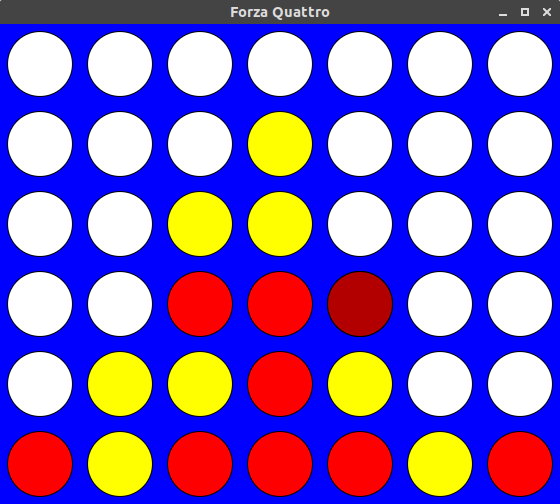
\includegraphics[width=.55\textwidth]{f4}
  \caption{The Four in a Row game created using piksel.}
\end{figure}

\section{Using piksel}

To make sure that you will be able to do the lab, we will first download and test the piksel library. Afterwards, you will be given information about few useful methods that you will need to create the four in a row application.

\subsection{Compiling the library}

Using a terminal, move to the main folder of the assignment and download piksel using:

\begin{center}
\ttfamily
git clone --recursive https://github.com/bernhardfritz/piksel.git
\end{center}

To test if everything works fine, create in the project root a new folder named \texttt{src}. Add the new file \texttt{piksel\string_example.cpp} and paste the following code inside it\footnote{The file can be copied directly from \texttt{solution/src/piksel\string_example.cpp}}:


\lstinputlisting[style=mycpp]{../solution/src/piksel_example.cpp}

To compile the code, add a \texttt{CMakeLists.txt} file inside the project root directory, and include the following lines of code\footnote{The name of the project corresponds to the Italian version of the game, feel free to name it differently.}:

\begin{lstlisting}[style=mycmake]
cmake_minimum_required(VERSION 3.1)
project(forza_quattro)

# use C++11 features
set(CMAKE_CXX_STANDARD 11)

# tell CMake to compile piksel as well
add_subdirectory(piksel)

# tell the compiler where to find piksel's headers
include_directories(piksel/src)

# compile the example
add_executable(piksel_example src/piksel_example.cpp)
target_link_libraries(piksel_example piksel)
\end{lstlisting}

Do not bother understanding it for now, we will come back to it in the next section. Time to compile: create a new folder named \texttt{build} and move inside it, then type the command \texttt{cmake~..} to start configuring. You might get an error concerning the version of CMake (piksel requires 3.12), but do not worry! The \href{https://bernhardfritz.github.io/piksel/#/gettingstarted/troubleshooting}{official solution} is to install the correct version of CMake, which does not require a lot of work. For simplicity, the steps are reported here:

\begin{center}
\begin{minipage}{.9\textwidth}
\begin{lstlisting}[style=myterm]
mkdir -p ~/programs_sources && cd ~/programs_sources
version=3.12
build=1
wget https://cmake.org/files/v$version/cmake-$version.$build.tar.gz
tar -xzvf cmake-$version.$build.tar.gz
cd cmake-$version.$build/
./bootstrap
make -j4
sudo make install
\end{lstlisting}
\end{minipage}
\end{center}

To check if the installation went fine, try to type \texttt{cmake --version} on your console: you should see the newly installed version 3.12.1. Also, as a good rule, do not delete the folder that contains the compiled CMake sources, \eg, \texttt{\textasciitilde/program\string_sources/cmake\string_3.12.1}. In fact, if in the future you wish to remove the installed version, it will suffice to move inside such directory and type \texttt{sudo make uninstall}. As a plus, from now on you can use the folder \texttt{program\string_sources} to install programs from their sources.

\begin{mdframed}[hidealllines=true,backgroundcolor=red!20]
  \underline{\textsc{Be careful}}: by default, the new CMake will be installed in \texttt{/usr/local}. If you have already a CMake binary installed there, the procedures above might override it completely. For a safer procedure, make a backup before typing \texttt{sudo make install}. You can do that simply by running:
  \begin{center}
    \ttfamily
    sudo cp -p /usr/local/bin/cmake.3.10.1
  \end{center}
  The example assumes you have CMake 3.10.1 installed, change it to reflect the correct version!
\end{mdframed}

A ``quick-n-dirty'' workaround is also possible: simply open the file \texttt{piksel/CMakeLists.txt} and change the required version of CMake to the one that you have, \eg, 3.1. Note that with this solution the build might fail completely or that some piksel's functionalities might not work as intended.

Coming back to compiling piksel, after a successful configuration type \texttt{make} to build the executable and finally \texttt{./piksel\string_example} to run it. You should see a rectangular window appearing in your screen, with a solid colored background. In addition, when moving the mouse inside the window, a white circle should be drawn following you. If so, then congratulations, piksel has been correctly compiled!




\subsection{Understanding piksel's fundamental classes}

Applications in piksel are rather simple: they all inherit from the base class \texttt{BaseApp}, which exposes a couple of virtual methods that can be overridden to customize the behavior of the program. In particular, the methods we are interested in are:

\begin{description}
  \item[\ttfamily BaseApp(int,int,std::string)] Constructor, takes the size (in pixels) of the window and optionally a string representing the ``title'' of the application.
  \item[\ttfamily virtual void setup()] Called once as soon as the application starts.
  \item[\ttfamily virtual void draw(piksel::Graphics\&)] Called repeatedly by the application, each call can be used to ``render'' a single frame. The \texttt{Graphics} object can be used to add shapes inside the window.
  \item[\ttfamily virtual void mousePressed(int)] Called when a mouse button is pushed down (not ``clicked''). The integer parameter allows to distinguish between different buttons on the mouse.
  \item[\ttfamily virtual void mouseMoved(int,int)] Executed when the mouse changes position inside the window. The two input variables correspond to the current horizontal and vertical coordinates (in pixels) of the device.
  \item[void run()] This is the ``entry-point'' of the application (generally invoked in \texttt{main}). You can think of it as a call to \texttt{setup} followed by an infinite loop that repeatedly calls \texttt{draw}.
\end{description}

The other fundamental class used in this library is \texttt{Graphics}, which is used to draw inside the canvas. We will not go into details, and we will just focus on few methods:

\begin{description}
  \item[void background(glm::vec4)] Allows to set the color of the background to the given one.
  \item[void ellipse(float,float,float,float)] Draws an ellipse in the specified coordinates (first two parameters of the function) with given width and height (third and fourth variables).
  \item[void fill(glm::vec4)] Changes the color used to draw shapes, such as ellipses.
  \item[void text(std::string,float,float)] Prints some text at the given coordinates.
  \item[void textSize(float)] Changes the size for following calls to \texttt{text}.
\end{description}

Finally, colors are all declared using the class \texttt{glm::vec4}, whose constructor accepts four \texttt{float} parameters, representing the RGBa (red, green, blue and alpha) components of the color, all normalized between 0 and 1.

Looking at the example code compiled in the previous section, it should be rather easy to understand what happens. First of all, we create a new class \texttt{App}, inheriting from \texttt{BaseApp}. The constructor simply initializes the canvas by calling the constructor of the base class. \texttt{App} has three private members: the background color of the canvas and the ``recorded'' mouse position. The color is initialized to a random one in the \texttt{setup} method. We also override the virtual method \texttt{mouseMoved}, whose default implementation is empty, so that the new coordinates of the mouse are saved whenever it is moved. Finally, the \texttt{draw} method will fill the background with the random color generated in \texttt{setup} and also draw a circle of fixed size in the recorded mouse position. To actually run the code, in the \texttt{main} method we create an instance of \texttt{App} and ``execute'' it by calling \texttt{start} (inherited from \texttt{BaseApp}).

Hoping that everything is clear up to this point, we are ready to start the actual assignment!



\section{Four in a Row}

Let's start by introducing the rules of the game:
\begin{itemize}
  \item A rectangular grid of $R\times C$ cells is initially empty
  \item Each of the two players is assigned a color, either red or yellow
  \item Players alternate in selecting one column out of the $C$ available ones and they are not allowed to pass (a choice must always be made)
  \item A fully filled column cannot be selected
  \item Once a column is selected, a chip is inserted in it reaching the lowest free cell
  \item The first player who aligns four or more chips in any direction (horizontal, vertical, diagonal) wins the game
\end{itemize}
With these rules in mind, it is decided to implement the game as follows:
\begin{itemize}
  \item An \emph{abstract} class \texttt{Player} provides the \emph{interface} for a player. It will expose a \emph{pure virtual method} called \texttt{choose} that asks to select a column. Concrete implementations of this class will define different strategies, \eg, using the mouse to select a column (human player) or randomly selecting a valid column (a very bad AI).
  \item The class \texttt{Board} will serve two objectives at the same time: on one hand, it will store and handle the grid by exposing methods to query/update cells content, and on the other hand it will take care of graphics management by inheriting from \texttt{BaseApp} and overriding some of its methods. 
\end{itemize}

In the following, you will be given some suggestions to implement these classes. As almost always in programming, there exist many different ways to accomplish the same task, and thus you might decide to use different strategies. If you feel like there is a better way to implement the code, you are encouraged to give it a try!






\subsection{Class \texttt{Board} - Basics}

This section concerns the creation of the basic functionalities of the \texttt{Board} class, \ie, those not requiring the class \texttt{Player}. While adding and implementing new methods, remember to compile and run the code frequently in order to spot errors as soon as possible.

First of all, define a new empty class that inherits from \texttt{piksel::BaseApp}. Create the header and source file in the usual way: declarations go in the \texttt{.h} file, while implementations (the instructions of each method) should be in the \texttt{.cpp}. Remember to add the proper \texttt{\#ifndef} \texttt{...} \texttt{\#define} guards and to include relevant headers.





\subsubsection{The \texttt{Cell} Enum}

In order to represent the content of a cell in the board, we will use an internal enum named \texttt{Cell}. Its values should reflect the possibility of a cell being empty or filled with a red/yellow chip. You can declare it -- \emph{inside} the class definition -- as:
\begin{center}
\begin{minipage}{.9\textwidth}
\begin{lstlisting}[style=mycpp,numbers=none]
enum class Cell {
  EMPTY,
  RED,
  YELLOW
};
\end{lstlisting}
\end{minipage}
\end{center}

Being an internal class of \texttt{Board}, it is accessible via the syntax \texttt{Board::Cell}, and one of its value by writing, \eg, \texttt{Board::Cell::EMPTY}. Remember to add the declaration in the \emph{public} scope of the class, so that external code fragments can use it as well.

\subsubsection{Member Variables}

To avoid using hard-coded numbers here and there in the code, let's store the geometric parameters of the grid inside two \emph{static} members:
\begin{center}
\begin{minipage}{.9\textwidth}
\begin{lstlisting}[style=mycpp,numbers=none]
static const int CELL_SIZE;
static const int CHIP_DIAMETER;
\end{lstlisting}
\end{minipage}
\end{center}
The former is used to store the size of the grid (or, equivalently, the distance between two chips) while the latter gives the diameter of a single chip (it should be smaller than the size of the cell). Remember to initialize them in the beginning of the \texttt{board.cpp} file!

In addition, we will need some variables to store the grid. We can do that by adding the following \emph{private} members:
\begin{center}
\begin{minipage}{.9\textwidth}
\begin{lstlisting}[style=mycpp,numbers=none]
const unsigned int rows_, cols_;
std::vector<Cell> grid_;
\end{lstlisting}
\end{minipage}
\end{center}
As their names suggest, \texttt{rows\string_} and \texttt{cols\string_} contain the size of the grid, \ie, $R$ and $C$. The content of the grid is stored in the vector \texttt{grid\string_}, whose size will be set later to $R\times C$. Note that we use a ``linear'' structure (the vector) to store a matrix-like content (the grid). This is a pretty common choice in programming, and we will see later how to provide utility methods to access its content in a simple way.

\subsubsection{Constructors}

Declare three constructors with the following signatures:
\begin{center}
\begin{minipage}{.9\textwidth}
\begin{lstlisting}[style=mycpp,numbers=none]
Board();
Board(unsigned int size);
Board(unsigned int rows, unsigned int columns);
\end{lstlisting}
\end{minipage}
\end{center}
The first one should build a $6\times 7$ grid using \emph{constructor delegation}. Similarly, the second version will generate a squared grid with \texttt{size} rows and columns. The last constructor is the one that actually performs all the initialization: it should call \texttt{BaseApp}'s constructor\footnote{The size of the canvas should be related to the number of rows and columns in the grid, as well as to the \texttt{CELL\string_SIZE}}, save the number of rows/columns in the grid and initialize \texttt{grid\string_} to the proper size, with all cells being initially empty.

Even with this thin definition, you can already try executing some code to start debugging the class. Create a new source file containing a \texttt{main} that instanciates a \texttt{Board} object and runs the application.

\subsubsection{Simple accessors}\label{sec:simple_accessors}

We can proceed by providing simple accessors to the grid properties. Add the following declarations to the public scope of your class:
\begin{center}
\begin{minipage}{.9\textwidth}
\begin{lstlisting}[style=mycpp,numbers=none]
const unsigned int& rows() const;
const unsigned int& cols() const;
const Cell& cell(unsigned int r, unsigned int c) const;
\end{lstlisting}
\end{minipage}
\end{center}
The first two methods should simply return the internal members \texttt{rows\string_} and \texttt{cols\string_}. Please note the \texttt{const} qualifiers both before and after the method declaration: do you understand why they are there? If not, ask the teacher!

The method \texttt{cell} should be used to simplify the access to elements contained inside the vector \texttt{grid\string_}. In practice, it should return the value of the cell located at the given row \texttt{r} and column \texttt{c}, and its implementation depends on how you choose to handle the content of the vector. To give an example, a matrix-like structure can be stored in a vector by writing it ``row by row'', also known as \href{https://en.wikipedia.org/wiki/Row-_and_column-major_order#Programming_languages_and_libraries}{row major ordering}. In this case, the index $k$ corresponding to a given row $i$ and column $j$ can be evaluated as $$k = i \times C + j$$


\subsubsection{Drawing the board}

We can now display the content of the grid, using the two methods below:
\begin{center}
\begin{minipage}{.9\textwidth}
\begin{lstlisting}[style=mycpp,numbers=none]
void cellCenter(
  unsigned int r,
  unsigned int c,
  float& x,
  float& y
);

void draw(piksel::Graphics& g) override;
\end{lstlisting}
\end{minipage}
\end{center}
Both methods can be put in the private scope of the class. The first one is an auxiliary method that takes as an input the row and column indices of a cell and evaluate the coordinates of its center in the canvas.

The method \texttt{draw} overrides \texttt{BaseApp}'s one and should render the grid. To do that, you can simply loop over all rows and columns of the grid and draw an ellipse for each cell depending on its content (use the methods \texttt{cell} and \texttt{cellCenter}, altogether with those provided by piksel's \texttt{Graphics} class).


\subsubsection{Additional cells methods}

This basic version of the \texttt{Board} class is almost finished. We just need two methods to facilitate accessing and changing the cells in the grid:
\begin{center}
\begin{minipage}{.9\textwidth}
\begin{lstlisting}[style=mycpp,numbers=none]
public: bool next(unsigned int c, unsigned int& r) const;
private: Cell& cell(unsigned int r, unsigned int c);
\end{lstlisting}
\end{minipage}
\end{center}
The method \texttt{next} takes the index \texttt{c} of a column and returns \texttt{false} if no additional chips can be inserted there. If the column has still some space instead, the index of the first free row (from the bottom of the grid!) is stored in \texttt{r} and \texttt{true} is returned instead.

The second method is almost identical to the \texttt{cell} accessor defined in \cref{sec:simple_accessors}. The difference is that the returned reference is not constant, \ie, its content can be changed. This is the main reason to put the method in the private scope: anybody can read the value of one cell, but we want the \texttt{Board} class only to be able to change the state of the grid.

Having added these methods, you can try to manually change the initial state of the grid in the constructor of the class. Use the method \texttt{next} to evaluate valid rows for the given columns and use \texttt{cell} to change their value. Clearly, this manual change is just for temporary testing and we will remove it in the next sections.




\subsection{Class \texttt{Player}}

Let's leave the \texttt{Board} class for a moment -- we will come back to it later -- so that we can start implementing the \texttt{Player} class. We will see in the following how to define it and how to implement new player types for our game.


\subsubsection{Protected member variables}

The attributes of the \texttt{Player} class will be just two, the color used by the player and a reference to the board used for the game:
\begin{center}
\begin{minipage}{.9\textwidth}
\begin{lstlisting}[style=mycpp,numbers=none]
Board::Cell color_;
Board& board_;
\end{lstlisting}
\end{minipage}
\end{center}
Thanks to the \texttt{Board} reference, the player will be able to query the current state of the grid and thus to make decisions for the following move.

Place the two variables in the \emph{protected} scope of the class, so that they are not directly accessible from outside, but still visible to children classes.

Finally, provide an accessor and a mutator for the attribute \texttt{color\string_}.


\subsubsection{Constructor and destructor}

Add a constructor that takes a reference to a \texttt{Board} instance. In the \texttt{.cpp} file, make sure to properly initialize the internal \texttt{board\string_} reference. In addition, add a virtual destructor as follows:
\begin{center}
\begin{minipage}{.9\textwidth}
\begin{lstlisting}[style=mycpp,numbers=none]
virtual ~Player() = default;
\end{lstlisting}
\end{minipage}
\end{center}
To understand the declaration, let's first say that writing \texttt{\textasciitilde Player()} \texttt{=} \texttt{default;} is equivalent to providing an empty destructor, \ie, a destructor whose code is just \texttt{\string{\string}}.\footnote{For this reason, you do not need to add the definition of the destructor in the \texttt{.cpp} file!} However, I believe it is clearer and nicer to write explicitly \texttt{\textasciitilde Player()} \texttt{=} \texttt{default;} rather than \texttt{\textasciitilde Player()} \texttt{\string{\string}}. That being said, having a virtual destructor is not always necessary, and in our specific case would not be mandatory. However, it is part of best practices to add a (even empty) virtual destructor \emph{whenever your class has at least one virtual method}. More information about this can be found in the C++ FAQ entry ``\href{https://isocpp.org/wiki/faq/virtual-functions#virtual-dtors}{\emph{When should my destructor be virtual?}}''. It is not a big deal if you do not fully understand this, but at least be aware that if you plan to do inheritance, there are chances that you will need to provide a virtual destructor to your base class, even if empty.


\subsubsection{Virtual methods}

Add the two following public virtual methods to the class:
\begin{center}
\begin{minipage}{.9\textwidth}
\begin{lstlisting}[style=mycpp,numbers=none]
virtual bool choose(unsigned int& col) = 0;
virtual void start() {}
\end{lstlisting}
\end{minipage}
\end{center}
The first one is a \emph{pure virtual} method, thus making the class \emph{abstract}. Its goal is to choose the next move by storing in \texttt{col} where to insert the chip. The method will return \texttt{true} if a choice is made, and \texttt{false} if the player ``needs more time to think'' (it will be useful when implementing a ``human'' player).

The method \texttt{start} can instead be useful to ``reset a player'' before starting a game -- a single player might play multiple times! However, a default (empty) implementation is already provided for simplicity: it is up to child classes to decide whether it is useful to override it.



\subsubsection{Wait method}

Finally, we can add a simple auxiliary function (make it as protected):
\begin{center}
\begin{minipage}{.9\textwidth}
\begin{lstlisting}[style=mycpp,numbers=none]
void wait(int ms);
\end{lstlisting}
\end{minipage}
\end{center}
The function should wait for the given amount of \texttt{ms} milliseconds. To implement it, you can use the \texttt{BaseApp}\texttt{::}\texttt{millis} method, which returns the elapsed time (in milliseconds) since the start of the application. Such pausing function will be useful when implementing ``AI players''.



\subsubsection{Class \texttt{RandomPlayer}}

We have enough tools now to implement our first (rather inefficient) player type. Create the class \texttt{RandomPlayer} inheriting from \texttt{Player}, and override the \texttt{choose} method so that a valid column is chosen at random. If all columns are full, the method should return \texttt{false} since a choice cannot be made!






\subsection{Class \texttt{Board} -- integrating players}

We can now add players to our ``Four in a Row'' game. We will need to introduce new members to the existing \texttt{Board} class, to store the player and to let him/her/it choose columns during the game.



\subsubsection{Adding players}

To add a player, let's start by including the relevant header and by adding two variables to the class \texttt{Board}:
\begin{center}
\begin{minipage}{.9\textwidth}
\begin{lstlisting}[style=mycpp,numbers=none]
Player* red_player_;
Player* yellow_player_;
\end{lstlisting}
\end{minipage}
\end{center}
Make sure to initialize the two pointers to \texttt{nullptr} in the constructor, so that in the beginning they point to a known invalid address -- they could otherwise contain any value and it would be impossible to know whether they are valid or not.

Note that if you compile the code you will almost certainly get a compilation error like:
\begin{center}
  \ttfamily
  error: `Player' does not name a type: Player* red\string_player\string_;
\end{center}
This is due to something that is (sometimes) denoted as ``circular dependency''. This happens when a class \texttt{A} uses/has a member of type \texttt{B}, which in turn uses/has a member of type \texttt{A}. The problem can be solved using a \emph{forward declaration}, which in our case corresponds to adding right before the declaration of \texttt{Board} the ``incomplete'' declaration of \texttt{Player}:
\begin{center}
\begin{minipage}{.9\textwidth}
\begin{lstlisting}[style=mycpp,numbers=none]
class Player; // forward declaration

class Board {
  ...
  // The compiler does not really know how the `Player' class works
  // but at least it now knows that something like that exists
  Player* red_player_;
};
\end{lstlisting}
\end{minipage}
\end{center}

Up to now, the pointers to the \texttt{Player} instances are simply \texttt{nullptr}. To allow assigning players properly, let's add the public method
\begin{center}
\begin{minipage}{.9\textwidth}
\begin{lstlisting}[style=mycpp,numbers=none]
void setPlayers(Player& red, Player& yellow);
\end{lstlisting}
\end{minipage}
\end{center}
which should copy the address of the two given objects into the internal pointers. Make sure to check that the addresses are different, \ie, that the user did not call \texttt{setPlayers(x,x)}. You can now modify the main program to include the players before the game starts.


\subsubsection{Making players choose}

Add two private member variables to \texttt{Board}:
\begin{center}
\begin{minipage}{.9\textwidth}
\begin{lstlisting}[style=mycpp,numbers=none]
bool red_playing_;
Cell winner_;
\end{lstlisting}
\end{minipage}
\end{center}
the former used to know whose turn it is now, the latter to know who is the winner (we can use \texttt{Cell::EMPTY} to indicate that no one won yet).

Now add the private method \texttt{void update()} which will be used to ask the current player to pick a column. To implement it, try to follow the given pseudo-code:
\begin{center}
\begin{minipage}{.9\textwidth}
\begin{lstlisting}[style=mycpp,numbers=none]
void Board::update() {
  // select the current player depending on the value of `red_playing_'
  // (store the active player in a reference called `p'
  
  // call p.choose(column): if it returns false, exit immediately
  
  // if a column was selected, check that it has space:
  // if not, throw an exception
  
  // get the row in which the chip should be inserted, then use
  // the method `cell' to insert the chip in the grid - the color
  // to be used is p.color()
  
  // TODO LATER: check if the player won
  
  // switch the current player
}
\end{lstlisting}
\end{minipage}
\end{center}

Finally, add the following at the very beginning of the \texttt{draw} method:
\begin{center}
\begin{minipage}{.9\textwidth}
\begin{lstlisting}[style=mycpp,numbers=none]
if(winner_ == Cell::EMPTY)
  update();
\end{lstlisting}
\end{minipage}
\end{center}
which ensures that, if no one won yet, the players are continuously asked to make a choice.




\subsubsection{Right before starting a game}

To make sure that everything is properly setup before starting a game, we can override the method \texttt{setup} from \texttt{BaseApp}. Inside it, you should do a couple of operations:

In addition, make the method assign the correct colors to the players, \eg, by calling \begin{center}
\begin{minipage}{.9\textwidth}
\begin{lstlisting}[style=mycpp,numbers=none]
void Board::setup() {
  // clear all the values in the grid, to make sure they are EMPTY
  
  // initialize red_playing_
  
  // initialize winner_
  
  // check that the Player pointers are not nullptr
  // (throw an exception if they are)
  
  // set the color of the red and yellow player
  // using Player::setColor
  
  // call Player::start
}
\end{lstlisting}
\end{minipage}
\end{center}

And that's it! Well... almost!


\subsubsection{Checking who won}

You can start the game with two random players, but they will keep on playing until the grid is entirely filled. This is because we did not check yet whether a player won after making a move. Go back to the \texttt{update} method, and try to figure out how to check if the current player won the game.

\underline{Hint}: you can try to use a recursive auxiliary function that counts how many cells of the same color there are in a given direction (left, left+up, up, right+up, right, \etc).

In addition, in the \texttt{draw} method you can add a message that says which player won (if any).




\subsubsection{Resetting the game with a ``click''}\label{sec:reset_game}

As the very last step of this basic implementation, let's add the ability to reset a game by a mouse click. We can easily do that by overriding the method \texttt{mousePressed}, so that whenever the mouse is pressed the game is reset (just by calling \texttt{setup}) if the game has ended.




\subsection{Support for human players}

To implement a nicer interface allowing a human to play the game, we will add few functionalities to the existing \texttt{Board} class. In particular, we will add support to handle mouse motion, mouse clicks and a ``preview mode'' to help visualizing the effect of the next move.


\subsubsection{Mouse motion support}

When a human is playing, he/she will use the mouse to decide in which column the chip should be placed. For this purpose, we can add the following to our \texttt{Board} class:
\begin{center}
\begin{minipage}{.9\textwidth}
\begin{lstlisting}[style=mycpp,numbers=none]
private: int mx_;
private: void mouseMoved(int x, int y) override;
public: unsigned int mouseColumn() const;
\end{lstlisting}
\end{minipage}
\end{center}
The variable \texttt{mx\string_} will store the current horizontal position of the mouse in the canvas, which can be updated inside \texttt{mouseMoved} (using the input variable x only). The method \texttt{mouseColumn} can instead be used to return the current column selected using the mouse. To obtain such column, you need to perform a very simple operation using \texttt{mx\string_} and \texttt{CELL\string_SIZE}.


\subsubsection{Handling mouse clicks}

Mouse clicks can be handled in a similar way, by adding the following members to our class:
\begin{center}
\begin{minipage}{.9\textwidth}
\begin{lstlisting}[style=mycpp,numbers=none]
private: bool mouse_pressed_;
public: bool mousePressed();
\end{lstlisting}
\end{minipage}
\end{center}
The variable \texttt{mouse\string_pressed\string_} can be set to \texttt{true} inside the \texttt{mousePressed(int)} method added in \cref{sec:reset_game} -- provided that the game is not reset! Then, the new method \texttt{mousePressed()} will return \texttt{true} if \texttt{mouse\string_pressed\string_} has been changed, and reset it to \texttt{false}. In practice, the method returns \texttt{true} if the mouse has been clicked at least once since its last call.


\subsubsection{Previewing a move}

We can implement a sort of ``move preview'' by adding few lines of code to our class:
\begin{center}
\begin{minipage}{.9\textwidth}
\begin{lstlisting}[style=mycpp,numbers=none]
private: unsigned int preview_col_;
public: void preview(unsigned int col);
\end{lstlisting}
\end{minipage}
\end{center}
The variable \texttt{preview\string_col\string_} can be used to store in which column we would like to place a chip, even if we are not sure about it yet -- and this is why we want to see a preview! To ``disable'' the preview, we can decide that if the variable above is greater than (or equal to) the number of columns, then the preview should not be shown. The method \texttt{preview} is used to change \texttt{preview\string_col\string_} to a desired column index.

To actually display the preview, we can add in the \texttt{draw} method few lines of code that will add an ellipse in the desired location. By setting the color to either dark red or dark yellow, the ``preview chip'' will be distinguishable from those that have already been placed in the grid.


\subsubsection{Adding the \texttt{HumanPlayer} class}

You can now define a human player by adding a new class \texttt{HumanPlayer} inheriting from \texttt{Player}. The only thing you need is to override the \texttt{choose} method, whose pseudo-code is reported below:
\begin{center}
\begin{minipage}{.9\textwidth}
\begin{lstlisting}[style=mycpp,numbers=none]
bool HumanPlayer::choose(unsigned int& col) {
  // get currently selected column from the board
  
  // if the column is not a valid index, exit returning false
  
  // if the selected column is full, exit returning false
  
  // if the mouse has been pressed, exit returning true
  
  // if the mouse has not been pressed: only show a preview
  // and finally exit returning false
}
\end{lstlisting}
\end{minipage}
\end{center}

Change the main program so that it allows a human player to challenge the ``random AI''.


\section*{What next?}

The assignment is over, but you can try to improve and/or extend the code in many ways. Some examples:
\begin{itemize}
  \item When a player wins, show which chips are aligned in a row
  \item Create new (hopefully more powerful) AIs
  \item Add a ``revert'' functionality to the game, allowing to cancel the last move(s) when the backspace key is pressed
\end{itemize}

Have fun, and happy coding!

\end{document}